\documentclass[twoside]{book}

% Packages required by doxygen
\usepackage{fixltx2e}
\usepackage{calc}
\usepackage{doxygen}
\usepackage[export]{adjustbox} % also loads graphicx
\usepackage{graphicx}
\usepackage[utf8]{inputenc}
\usepackage{makeidx}
\usepackage{multicol}
\usepackage{multirow}
\PassOptionsToPackage{warn}{textcomp}
\usepackage{textcomp}
\usepackage[nointegrals]{wasysym}
\usepackage[table]{xcolor}

% Font selection
\usepackage[T1]{fontenc}
\usepackage[scaled=.90]{helvet}
\usepackage{courier}
\usepackage{amssymb}
\usepackage{sectsty}
\renewcommand{\familydefault}{\sfdefault}
\allsectionsfont{%
  \fontseries{bc}\selectfont%
  \color{darkgray}%
}
\renewcommand{\DoxyLabelFont}{%
  \fontseries{bc}\selectfont%
  \color{darkgray}%
}
\newcommand{\+}{\discretionary{\mbox{\scriptsize$\hookleftarrow$}}{}{}}

% Page & text layout
\usepackage{geometry}
\geometry{%
  a4paper,%
  top=2.5cm,%
  bottom=2.5cm,%
  left=2.5cm,%
  right=2.5cm%
}
\tolerance=750
\hfuzz=15pt
\hbadness=750
\setlength{\emergencystretch}{15pt}
\setlength{\parindent}{0cm}
\setlength{\parskip}{3ex plus 2ex minus 2ex}
\makeatletter
\renewcommand{\paragraph}{%
  \@startsection{paragraph}{4}{0ex}{-1.0ex}{1.0ex}{%
    \normalfont\normalsize\bfseries\SS@parafont%
  }%
}
\renewcommand{\subparagraph}{%
  \@startsection{subparagraph}{5}{0ex}{-1.0ex}{1.0ex}{%
    \normalfont\normalsize\bfseries\SS@subparafont%
  }%
}
\makeatother

% Headers & footers
\usepackage{fancyhdr}
\pagestyle{fancyplain}
\fancyhead[LE]{\fancyplain{}{\bfseries\thepage}}
\fancyhead[CE]{\fancyplain{}{}}
\fancyhead[RE]{\fancyplain{}{\bfseries\leftmark}}
\fancyhead[LO]{\fancyplain{}{\bfseries\rightmark}}
\fancyhead[CO]{\fancyplain{}{}}
\fancyhead[RO]{\fancyplain{}{\bfseries\thepage}}
\fancyfoot[LE]{\fancyplain{}{}}
\fancyfoot[CE]{\fancyplain{}{}}
\fancyfoot[RE]{\fancyplain{}{\bfseries\scriptsize Generated by Doxygen }}
\fancyfoot[LO]{\fancyplain{}{\bfseries\scriptsize Generated by Doxygen }}
\fancyfoot[CO]{\fancyplain{}{}}
\fancyfoot[RO]{\fancyplain{}{}}
\renewcommand{\footrulewidth}{0.4pt}
\renewcommand{\chaptermark}[1]{%
  \markboth{#1}{}%
}
\renewcommand{\sectionmark}[1]{%
  \markright{\thesection\ #1}%
}

% Indices & bibliography
\usepackage{natbib}
\usepackage[titles]{tocloft}
\setcounter{tocdepth}{3}
\setcounter{secnumdepth}{5}
\makeindex

% Hyperlinks (required, but should be loaded last)
\usepackage{ifpdf}
\ifpdf
  \usepackage[pdftex,pagebackref=true]{hyperref}
\else
  \usepackage[ps2pdf,pagebackref=true]{hyperref}
\fi
\hypersetup{%
  colorlinks=true,%
  linkcolor=blue,%
  citecolor=blue,%
  unicode%
}

% Custom commands
\newcommand{\clearemptydoublepage}{%
  \newpage{\pagestyle{empty}\cleardoublepage}%
}

\usepackage{caption}
\captionsetup{labelsep=space,justification=centering,font={bf},singlelinecheck=off,skip=4pt,position=top}

%===== C O N T E N T S =====

\begin{document}

% Titlepage & ToC
\hypersetup{pageanchor=false,
             bookmarksnumbered=true,
             pdfencoding=unicode
            }
\pagenumbering{alph}
\begin{titlepage}
\vspace*{7cm}
\begin{center}%
{\Large Coarse\+Graining\+Advanced }\\
\vspace*{1cm}
{\large Generated by Doxygen 1.8.13}\\
\end{center}
\end{titlepage}
\clearemptydoublepage
\pagenumbering{roman}
\tableofcontents
\clearemptydoublepage
\pagenumbering{arabic}
\hypersetup{pageanchor=true}

%--- Begin generated contents ---
\chapter{Class Index}
\section{Class List}
Here are the classes, structs, unions and interfaces with brief descriptions\+:\begin{DoxyCompactList}
\item\contentsline{section}{\hyperlink{classCGPoint}{C\+G\+Point} \\*Coarse graining point }{\pageref{classCGPoint}}{}
\item\contentsline{section}{\hyperlink{classCoarsing}{Coarsing} \\*Main Coarse graining class }{\pageref{classCoarsing}}{}
\item\contentsline{section}{\hyperlink{structData}{Data} \\*\hyperlink{structData}{Data} structure handling point data and contact data }{\pageref{structData}}{}
\item\contentsline{section}{\hyperlink{structField}{Field} \\*Contains \hyperlink{structField}{Field} informations }{\pageref{structField}}{}
\end{DoxyCompactList}

\chapter{Class Documentation}
\hypertarget{classCGPoint}{}\section{C\+G\+Point Class Reference}
\label{classCGPoint}\index{C\+G\+Point@{C\+G\+Point}}


Coarse graining point.  




{\ttfamily \#include $<$Coarsing.\+h$>$}

\subsection*{Public Member Functions}
\begin{DoxyCompactItemize}
\item 
\mbox{\Hypertarget{classCGPoint_a85026786569ae92db296a062327322bc}\label{classCGPoint_a85026786569ae92db296a062327322bc}} 
{\bfseries C\+G\+Point} (int dd, v1d loc)
\end{DoxyCompactItemize}
\subsection*{Public Attributes}
\begin{DoxyCompactItemize}
\item 
\mbox{\Hypertarget{classCGPoint_ad0fd06c53bc917bdf91abbbdb4b8e4c3}\label{classCGPoint_ad0fd06c53bc917bdf91abbbdb4b8e4c3}} 
v2d \hyperlink{classCGPoint_ad0fd06c53bc917bdf91abbbdb4b8e4c3}{fields}
\begin{DoxyCompactList}\small\item\em 1st dimension is time, second are fields \end{DoxyCompactList}\item 
\mbox{\Hypertarget{classCGPoint_a8b3032ef9cfc6f32d1cab9aa912ce82d}\label{classCGPoint_a8b3032ef9cfc6f32d1cab9aa912ce82d}} 
v1d \hyperlink{classCGPoint_a8b3032ef9cfc6f32d1cab9aa912ce82d}{location}
\begin{DoxyCompactList}\small\item\em Location of the coarse graining point. \end{DoxyCompactList}\item 
\mbox{\Hypertarget{classCGPoint_a50e3237ed6a858bd62b8196f0cff2332}\label{classCGPoint_a50e3237ed6a858bd62b8196f0cff2332}} 
vector$<$ int $>$ \hyperlink{classCGPoint_a50e3237ed6a858bd62b8196f0cff2332}{neighbors}
\begin{DoxyCompactList}\small\item\em All the neighbors of the point given the window. 1st index is the point itself. \end{DoxyCompactList}\end{DoxyCompactItemize}


\subsection{Detailed Description}
Coarse graining point. 

The documentation for this class was generated from the following file\+:\begin{DoxyCompactItemize}
\item 
Coarsing.\+h\end{DoxyCompactItemize}

\hypertarget{classCoarsing}{}\section{Coarsing Class Reference}
\label{classCoarsing}\index{Coarsing@{Coarsing}}


Main Coarse graining class.  




{\ttfamily \#include $<$Coarsing.\+h$>$}



Collaboration diagram for Coarsing\+:\nopagebreak
\begin{figure}[H]
\begin{center}
\leavevmode
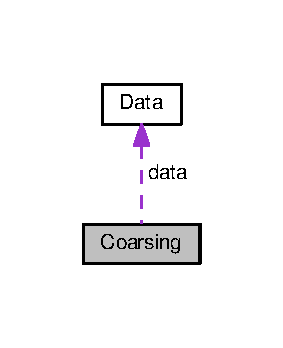
\includegraphics[width=136pt]{classCoarsing__coll__graph}
\end{center}
\end{figure}
\subsection*{Public Member Functions}
\begin{DoxyCompactItemize}
\item 
\mbox{\Hypertarget{classCoarsing_a11132c6d00ff7325439fbf22f0123f14}\label{classCoarsing_a11132c6d00ff7325439fbf22f0123f14}} 
{\bfseries Coarsing} (int dd, v1i nnpt, v2d bbox, double ww, int T)
\item 
\mbox{\Hypertarget{classCoarsing_a55274243000bb927b512fd2d74d19cb9}\label{classCoarsing_a55274243000bb927b512fd2d74d19cb9}} 
int {\bfseries get\+\_\+id} (string nm)
\item 
\mbox{\Hypertarget{classCoarsing_a8ea9edcad1f8b08efa58bff025d5632d}\label{classCoarsing_a8ea9edcad1f8b08efa58bff025d5632d}} 
int {\bfseries grid\+\_\+generate} ()
\item 
\mbox{\Hypertarget{classCoarsing_ab6a0de9ae7a9d780cd1e8496e6dead3e}\label{classCoarsing_ab6a0de9ae7a9d780cd1e8496e6dead3e}} 
int {\bfseries grid\+\_\+neighbour} ()
\item 
\mbox{\Hypertarget{classCoarsing_a9d8a9b0c9393ffa0e28e30a7baf47e8f}\label{classCoarsing_a9d8a9b0c9393ffa0e28e30a7baf47e8f}} 
int {\bfseries grid\+\_\+setfields} ()
\item 
\mbox{\Hypertarget{classCoarsing_a1e90778213173410a73cda8d0335ad04}\label{classCoarsing_a1e90778213173410a73cda8d0335ad04}} 
v1d {\bfseries grid\+\_\+getfields} ()
\item 
\mbox{\Hypertarget{classCoarsing_ad9e3c512dd13cd0448c4269d1a4ee371}\label{classCoarsing_ad9e3c512dd13cd0448c4269d1a4ee371}} 
int {\bfseries find\+\_\+closest} (int id)
\item 
\mbox{\Hypertarget{classCoarsing_a4d71faafcbf3955a2c1ea105f940c17a}\label{classCoarsing_a4d71faafcbf3955a2c1ea105f940c17a}} 
int {\bfseries find\+\_\+closest\+\_\+pq} (int id)
\item 
\mbox{\Hypertarget{classCoarsing_aa280ef8c110e4a95f21e001cac5af882}\label{classCoarsing_aa280ef8c110e4a95f21e001cac5af882}} 
v1d {\bfseries interpolate\+\_\+vel} (int id)
\item 
\mbox{\Hypertarget{classCoarsing_a6b31e948d1213f1a8f31b9d85d75d65c}\label{classCoarsing_a6b31e948d1213f1a8f31b9d85d75d65c}} 
v1d {\bfseries interpolate\+\_\+rot} (int id)
\item 
\mbox{\Hypertarget{classCoarsing_ae61c76b2253b2e9b68878e722b7df6df}\label{classCoarsing_ae61c76b2253b2e9b68878e722b7df6df}} 
v1d {\bfseries interpolate\+\_\+vel\+\_\+nearest} (int id)
\item 
\mbox{\Hypertarget{classCoarsing_a3a8756a170e75cea83e9dddfe5b2fe57}\label{classCoarsing_a3a8756a170e75cea83e9dddfe5b2fe57}} 
v1d {\bfseries interpolate\+\_\+rot\+\_\+nearest} (int id)
\item 
double \hyperlink{classCoarsing_ae58a2ff869a21d6590983c47f45c302f}{window} (double r)
\item 
\mbox{\Hypertarget{classCoarsing_a9e816e036f21344f6cbce59f915a378c}\label{classCoarsing_a9e816e036f21344f6cbce59f915a378c}} 
double \hyperlink{classCoarsing_a9e816e036f21344f6cbce59f915a378c}{window\+\_\+int} (v1d r1, v1d lpq, v1d x)
\begin{DoxyCompactList}\small\item\em Numerical integration\+: not implemented. \end{DoxyCompactList}\item 
\mbox{\Hypertarget{classCoarsing_a592f32474e5d1780964dbc963590b888}\label{classCoarsing_a592f32474e5d1780964dbc963590b888}} 
double \hyperlink{classCoarsing_a592f32474e5d1780964dbc963590b888}{window\+\_\+int} (double r1, double r2)
\begin{DoxyCompactList}\small\item\em Overload to avoid integration ... \end{DoxyCompactList}\item 
\mbox{\Hypertarget{classCoarsing_a710e52466854458219f2187059d003e4}\label{classCoarsing_a710e52466854458219f2187059d003e4}} 
double {\bfseries window\+\_\+avg} (double r1, double r2)
\item 
\mbox{\Hypertarget{classCoarsing_a7c0f9ee3ec935f461c6af5e2d8ff407d}\label{classCoarsing_a7c0f9ee3ec935f461c6af5e2d8ff407d}} 
double {\bfseries Lucy} (double r)
\item 
\mbox{\Hypertarget{classCoarsing_a0439f0c3d74f73da7d6942508ef55d0b}\label{classCoarsing_a0439f0c3d74f73da7d6942508ef55d0b}} 
double {\bfseries normdiff} (v1d a, v1d b)
\item 
\mbox{\Hypertarget{classCoarsing_a41a64f445a65ae8fa6355cf75e095779}\label{classCoarsing_a41a64f445a65ae8fa6355cf75e095779}} 
int \hyperlink{classCoarsing_a41a64f445a65ae8fa6355cf75e095779}{pass\+\_\+1} ()
\begin{DoxyCompactList}\small\item\em Coarse-\/grain anything based on particles (not contacts) which does not need fluctuating quantities. \end{DoxyCompactList}\item 
\mbox{\Hypertarget{classCoarsing_a0556e88442645cf2def6f9ce918b9bb3}\label{classCoarsing_a0556e88442645cf2def6f9ce918b9bb3}} 
int \hyperlink{classCoarsing_a0556e88442645cf2def6f9ce918b9bb3}{pass\+\_\+2} ()
\begin{DoxyCompactList}\small\item\em Coarse-\/grain anything based on particles (not contacts) which needs fluctuating quantities (call the compute\+\_\+fluc\+\_\+ functions before) \end{DoxyCompactList}\item 
\mbox{\Hypertarget{classCoarsing_ac2ae89b569d5d21ff2f54798021d366a}\label{classCoarsing_ac2ae89b569d5d21ff2f54798021d366a}} 
int \hyperlink{classCoarsing_ac2ae89b569d5d21ff2f54798021d366a}{pass\+\_\+3} ()
\begin{DoxyCompactList}\small\item\em Coarse-\/grain anything based on contact informations. \end{DoxyCompactList}\item 
\mbox{\Hypertarget{classCoarsing_ab5c674784326a7be061683edc160753a}\label{classCoarsing_ab5c674784326a7be061683edc160753a}} 
int {\bfseries compute\+\_\+fluc\+\_\+vel} ()
\item 
\mbox{\Hypertarget{classCoarsing_a2fa1d870e2b81306b5cc67886b35d928}\label{classCoarsing_a2fa1d870e2b81306b5cc67886b35d928}} 
int {\bfseries compute\+\_\+fluc\+\_\+rot} ()
\item 
\mbox{\Hypertarget{classCoarsing_accc475e5888ec7a03a26b2354716a41d}\label{classCoarsing_accc475e5888ec7a03a26b2354716a41d}} 
int \hyperlink{classCoarsing_accc475e5888ec7a03a26b2354716a41d}{distance} (int id, v1d loc)
\begin{DoxyCompactList}\small\item\em function for mixed particle id / vector informations. \end{DoxyCompactList}\end{DoxyCompactItemize}
\subsection*{Public Attributes}
\begin{DoxyCompactItemize}
\item 
\mbox{\Hypertarget{classCoarsing_a88086b32fb8eb340560c00ad3f132937}\label{classCoarsing_a88086b32fb8eb340560c00ad3f132937}} 
int \hyperlink{classCoarsing_a88086b32fb8eb340560c00ad3f132937}{d}
\begin{DoxyCompactList}\small\item\em Number of dimensions. \end{DoxyCompactList}\item 
\mbox{\Hypertarget{classCoarsing_a0f4ae1846092ee42c3cc0b55cec85ed1}\label{classCoarsing_a0f4ae1846092ee42c3cc0b55cec85ed1}} 
int \hyperlink{classCoarsing_a0f4ae1846092ee42c3cc0b55cec85ed1}{Npt}
\begin{DoxyCompactList}\small\item\em Number of coarse graining points. \end{DoxyCompactList}\item 
\mbox{\Hypertarget{classCoarsing_a49f5477a50665dabd7c8d6ee05fbfb89}\label{classCoarsing_a49f5477a50665dabd7c8d6ee05fbfb89}} 
int \hyperlink{classCoarsing_a49f5477a50665dabd7c8d6ee05fbfb89}{Time}
\begin{DoxyCompactList}\small\item\em Total timesteps. \end{DoxyCompactList}\item 
\mbox{\Hypertarget{classCoarsing_a820ee3cdc5a2f3a10fdfb295abd72f9a}\label{classCoarsing_a820ee3cdc5a2f3a10fdfb295abd72f9a}} 
int \hyperlink{classCoarsing_a820ee3cdc5a2f3a10fdfb295abd72f9a}{cT}
\begin{DoxyCompactList}\small\item\em Current timestep. \end{DoxyCompactList}\item 
\mbox{\Hypertarget{classCoarsing_a4f64442e557dfbff555f0d8a5e2c7ffa}\label{classCoarsing_a4f64442e557dfbff555f0d8a5e2c7ffa}} 
double {\bfseries w}
\item 
\mbox{\Hypertarget{classCoarsing_a1cc37fdd5e18d1a53c4d3e60be2b3c43}\label{classCoarsing_a1cc37fdd5e18d1a53c4d3e60be2b3c43}} 
double \hyperlink{classCoarsing_a1cc37fdd5e18d1a53c4d3e60be2b3c43}{cutoff}
\begin{DoxyCompactList}\small\item\em CG width, and cutoff. \end{DoxyCompactList}\item 
\mbox{\Hypertarget{classCoarsing_a17b179f56085f3f9a172e4591fc21a2b}\label{classCoarsing_a17b179f56085f3f9a172e4591fc21a2b}} 
vector$<$ class \hyperlink{classCGPoint}{C\+G\+Point} $>$ \hyperlink{classCoarsing_a17b179f56085f3f9a172e4591fc21a2b}{C\+GP}
\begin{DoxyCompactList}\small\item\em List of Coarse Graining points. \end{DoxyCompactList}\item 
\mbox{\Hypertarget{classCoarsing_adb12a0d3e3ae6634cf8801555f0afedd}\label{classCoarsing_adb12a0d3e3ae6634cf8801555f0afedd}} 
vector$<$ int $>$ \hyperlink{classCoarsing_adb12a0d3e3ae6634cf8801555f0afedd}{npt}
\begin{DoxyCompactList}\small\item\em Number of points per dimension. \end{DoxyCompactList}\item 
\mbox{\Hypertarget{classCoarsing_ad50b41450dd51c366ecb4fd1ec07e03d}\label{classCoarsing_ad50b41450dd51c366ecb4fd1ec07e03d}} 
vector$<$ int $>$ \hyperlink{classCoarsing_ad50b41450dd51c366ecb4fd1ec07e03d}{nptcum}
\begin{DoxyCompactList}\small\item\em Cumulated number of points per dimensions (usefull for quick finding of the closest CG for a grain) \end{DoxyCompactList}\item 
\mbox{\Hypertarget{classCoarsing_abf3938c073fe57b4515bd54897c77d69}\label{classCoarsing_abf3938c073fe57b4515bd54897c77d69}} 
v1d {\bfseries dx}
\item 
\mbox{\Hypertarget{classCoarsing_a693207f9b72e42b89e1d68b9a6259fa6}\label{classCoarsing_a693207f9b72e42b89e1d68b9a6259fa6}} 
v2d {\bfseries box}
\item 
\mbox{\Hypertarget{classCoarsing_a71f3970db217286403591f34bd51c2da}\label{classCoarsing_a71f3970db217286403591f34bd51c2da}} 
unsigned int \hyperlink{classCoarsing_a71f3970db217286403591f34bd51c2da}{flags}
\begin{DoxyCompactList}\small\item\em Flags deciding which fields to coarse-\/grain. \end{DoxyCompactList}\item 
\mbox{\Hypertarget{classCoarsing_aa2fe878237d61cfea5421bd433e1210d}\label{classCoarsing_aa2fe878237d61cfea5421bd433e1210d}} 
vector$<$ string $>$ \hyperlink{classCoarsing_aa2fe878237d61cfea5421bd433e1210d}{Fields}
\begin{DoxyCompactList}\small\item\em Flagged field names. \end{DoxyCompactList}\item 
\mbox{\Hypertarget{classCoarsing_a07ec285bd11033d10f7a27a38bd5fd62}\label{classCoarsing_a07ec285bd11033d10f7a27a38bd5fd62}} 
vector$<$ int $>$ \hyperlink{classCoarsing_a07ec285bd11033d10f7a27a38bd5fd62}{Fidx}
\begin{DoxyCompactList}\small\item\em Where the fields is referenced in the fields vector in the \hyperlink{classCGPoint}{C\+G\+Point}. -\/1 if not flagged. \end{DoxyCompactList}\item 
\mbox{\Hypertarget{classCoarsing_a56e5de2d000122cd6054017025e9634b}\label{classCoarsing_a56e5de2d000122cd6054017025e9634b}} 
vector$<$ struct \hyperlink{structField}{Field} $>$ \hyperlink{classCoarsing_a56e5de2d000122cd6054017025e9634b}{F\+I\+E\+L\+DS}
\begin{DoxyCompactList}\small\item\em All allowed fields (initialized in grid\+\_\+getfields) \end{DoxyCompactList}\item 
\mbox{\Hypertarget{classCoarsing_a884bf9b4d9d9f5ae124c13cb353540f3}\label{classCoarsing_a884bf9b4d9d9f5ae124c13cb353540f3}} 
struct \hyperlink{structData}{Data} {\bfseries data}
\end{DoxyCompactItemize}


\subsection{Detailed Description}
Main Coarse graining class. 

\subsection{Member Function Documentation}
\mbox{\Hypertarget{classCoarsing_ae58a2ff869a21d6590983c47f45c302f}\label{classCoarsing_ae58a2ff869a21d6590983c47f45c302f}} 
\index{Coarsing@{Coarsing}!window@{window}}
\index{window@{window}!Coarsing@{Coarsing}}
\subsubsection{\texorpdfstring{window()}{window()}}
{\footnotesize\ttfamily double Coarsing\+::window (\begin{DoxyParamCaption}\item[{double}]{r }\end{DoxyParamCaption})\hspace{0.3cm}{\ttfamily [inline]}}

Windowing functions 

The documentation for this class was generated from the following files\+:\begin{DoxyCompactItemize}
\item 
Coarsing.\+h\item 
Coarsing.\+cpp\end{DoxyCompactItemize}

\hypertarget{structData}{}\section{Data Struct Reference}
\label{structData}\index{Data@{Data}}


\hyperlink{structData}{Data} structure handling point data and contact data.  




{\ttfamily \#include $<$Coarsing.\+h$>$}

\subsection*{Public Member Functions}
\begin{DoxyCompactItemize}
\item 
\mbox{\Hypertarget{structData_a52baee43793f5f03088eb32a36f4c6fb}\label{structData_a52baee43793f5f03088eb32a36f4c6fb}} 
int \hyperlink{structData_a52baee43793f5f03088eb32a36f4c6fb}{random\+\_\+test} (int N, int Ncf, int d, v2d box)
\begin{DoxyCompactList}\small\item\em Randomly fill the data structure. \end{DoxyCompactList}\item 
\mbox{\Hypertarget{structData_aba0bdd673b8a3d0401deb7da3e479735}\label{structData_aba0bdd673b8a3d0401deb7da3e479735}} 
int \hyperlink{structData_aba0bdd673b8a3d0401deb7da3e479735}{compute\+\_\+lpq} (int d)
\begin{DoxyCompactList}\small\item\em Compute lpq from contact id\textquotesingle{}s and atom locations. \end{DoxyCompactList}\end{DoxyCompactItemize}
\subsection*{Public Attributes}
\begin{DoxyCompactItemize}
\item 
\mbox{\Hypertarget{structData_a3be03de44986fc55905076acc5cdae2e}\label{structData_a3be03de44986fc55905076acc5cdae2e}} 
int {\bfseries N}
\item 
\mbox{\Hypertarget{structData_a50ac6cb209a74ccda8482434f27dad76}\label{structData_a50ac6cb209a74ccda8482434f27dad76}} 
double $\ast$ {\bfseries mass}
\item 
\mbox{\Hypertarget{structData_a24e794ed02025d5f4bb90d223d18a909}\label{structData_a24e794ed02025d5f4bb90d223d18a909}} 
double $\ast$ {\bfseries Imom}
\item 
\mbox{\Hypertarget{structData_a64e7c2a261c99a49c6a069a549c1de42}\label{structData_a64e7c2a261c99a49c6a069a549c1de42}} 
vector$<$ double $\ast$ $>$ {\bfseries pos}
\item 
\mbox{\Hypertarget{structData_ad9eb9c715b1138b189d0b837807a9269}\label{structData_ad9eb9c715b1138b189d0b837807a9269}} 
vector$<$ double $\ast$ $>$ {\bfseries vel}
\item 
\mbox{\Hypertarget{structData_a1cbe3b0b910376fe41418a80e8884f35}\label{structData_a1cbe3b0b910376fe41418a80e8884f35}} 
vector$<$ double $\ast$ $>$ {\bfseries omega}
\item 
\mbox{\Hypertarget{structData_a9943c2f12cbe674a2660d5e370ad6192}\label{structData_a9943c2f12cbe674a2660d5e370ad6192}} 
v2d {\bfseries vel\+\_\+fluc}
\item 
\mbox{\Hypertarget{structData_ac752e81ef5cfd30eb36d0135ddc3ce9c}\label{structData_ac752e81ef5cfd30eb36d0135ddc3ce9c}} 
v2d \hyperlink{structData_ac752e81ef5cfd30eb36d0135ddc3ce9c}{rot\+\_\+fluc}
\begin{DoxyCompactList}\small\item\em Should not be externally provided but calculated, using the function {\itshape Coarsing\+::compute\+\_\+fluc\+\_\+vel()} \end{DoxyCompactList}\item 
\mbox{\Hypertarget{structData_a783cd6858ac404d58cd9c3087554e741}\label{structData_a783cd6858ac404d58cd9c3087554e741}} 
int {\bfseries Ncf}
\item 
\mbox{\Hypertarget{structData_a8e4044c32ca108735ac12f42be2ca7c1}\label{structData_a8e4044c32ca108735ac12f42be2ca7c1}} 
double $\ast$ {\bfseries id1}
\item 
\mbox{\Hypertarget{structData_aceab4d0bbe0b13734353bd1a67172485}\label{structData_aceab4d0bbe0b13734353bd1a67172485}} 
double $\ast$ {\bfseries id2}
\item 
\mbox{\Hypertarget{structData_a3cf4988534226aa1a566dfffb629f473}\label{structData_a3cf4988534226aa1a566dfffb629f473}} 
vector$<$ double $\ast$ $>$ {\bfseries pospq}
\item 
\mbox{\Hypertarget{structData_aa46a77763360df63a36f61d06ffb339b}\label{structData_aa46a77763360df63a36f61d06ffb339b}} 
vector$<$ double $\ast$ $>$ {\bfseries lpq}
\item 
\mbox{\Hypertarget{structData_a486a5f50a69db7164ab0304464028935}\label{structData_a486a5f50a69db7164ab0304464028935}} 
vector$<$ double $\ast$ $>$ {\bfseries fpq}
\item 
\mbox{\Hypertarget{structData_a2f41a3378af42030c55ea80b7027e9da}\label{structData_a2f41a3378af42030c55ea80b7027e9da}} 
vector$<$ double $\ast$ $>$ {\bfseries mpq}
\item 
\mbox{\Hypertarget{structData_ab25c53d90730b3488150cad41641c5d6}\label{structData_ab25c53d90730b3488150cad41641c5d6}} 
vector$<$ double $\ast$ $>$ {\bfseries mqp}
\end{DoxyCompactItemize}


\subsection{Detailed Description}
\hyperlink{structData}{Data} structure handling point data and contact data. 

The documentation for this struct was generated from the following files\+:\begin{DoxyCompactItemize}
\item 
Coarsing.\+h\item 
Coarsing.\+cpp\end{DoxyCompactItemize}

\hypertarget{structField}{}\section{Field Struct Reference}
\label{structField}\index{Field@{Field}}


Contains \hyperlink{structField}{Field} informations.  




{\ttfamily \#include $<$Coarsing.\+h$>$}

\subsection*{Public Attributes}
\begin{DoxyCompactItemize}
\item 
\mbox{\Hypertarget{structField_aac7e5b0b2e4c87d0ef057b71ea5fed97}\label{structField_aac7e5b0b2e4c87d0ef057b71ea5fed97}} 
int {\bfseries flag}
\item 
\mbox{\Hypertarget{structField_ab285d25456aca13adb626a89208d3dc2}\label{structField_ab285d25456aca13adb626a89208d3dc2}} 
string {\bfseries name}
\item 
\mbox{\Hypertarget{structField_a64da0458381eb5ef333274b4d5fa416e}\label{structField_a64da0458381eb5ef333274b4d5fa416e}} 
string {\bfseries type}
\end{DoxyCompactItemize}


\subsection{Detailed Description}
Contains \hyperlink{structField}{Field} informations. 

The documentation for this struct was generated from the following file\+:\begin{DoxyCompactItemize}
\item 
Coarsing.\+h\end{DoxyCompactItemize}

%--- End generated contents ---

% Index
\backmatter
\newpage
\phantomsection
\clearemptydoublepage
\addcontentsline{toc}{chapter}{Index}
\printindex

\end{document}
